\section{A daughter gluon from a parent quark}
\begin{figure}[ht!]
\centering
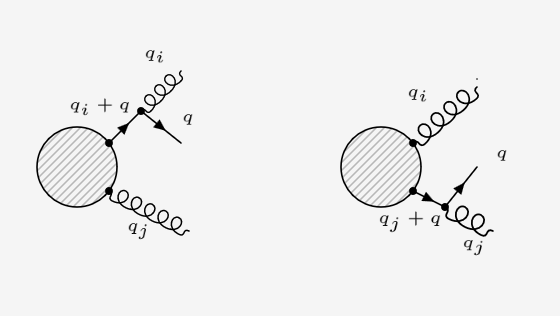
\includegraphics[width=0.85\textwidth]{images/GQ/GQDiagrams.png}
\end{figure}


\begin{figure}[ht!]
\centering
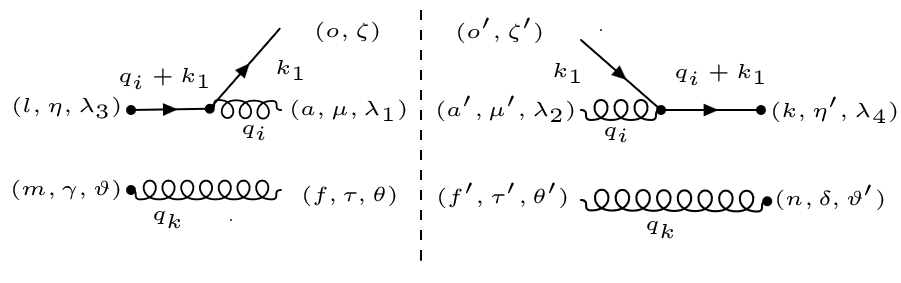
\includegraphics[scale=0.7]{images/GQ/M1Squer.png}
\end{figure}

\begin{equation}
\begin{split}
|M_1|^2=-\frac{{g_s}^2 {[T^{a^{\prime}}]_k}^{o^{\prime}} {[T^a]_{o}}^{l}}{4(k_1 \cdot q_i)(k_1 \cdot q_i)}[(\not{q_i}+\not{k_1}) {\gamma}_{{\mu}}\not{k_1}\:{\gamma}^{\mu}(\not{q_i}+\not{k_1})\:][-{g^{\delta}}_{\gamma}]
\end{split}
\end{equation}

\begin{equation}
\begin{split}
|M_1|^2=-(2-d)\frac{{g_s}^2 {[T^{a^{\prime}}]_k}^{o^{\prime}} {[T^a]_{o}}^{l}}{4(k_1 \cdot q_i)(k_1 \cdot q_i)}[(\not{q_i}+\not{k_1}) \not{k_1}(\not{q_i}+\not{k_1})\:][-{g^{\delta}}_{\gamma}]
\end{split}
\end{equation}

\begin{equation}
\begin{split}
|M_1|^2=-(2-d)\frac{{g_s}^2 {[T^{a^{\prime}}]_k}^{o^{\prime}} {[T^a]_{o}}^{l}}{2(k_1 \cdot q_i)}[\not{q_i}][-{g^{\delta}}_{\gamma}]
\end{split}
\end{equation}

\begin{equation}
\begin{split}
|M_1|^2=-(2-d)\frac{{g_s}^2 C_F}{2y\:p_i \cdot Q}
[(\alpha_1 -y\beta_1(\frac{Q^2}{2p_i \cdot Q})) \not{p_i} + y\beta_1\not{Q} + \sqrt{y\alpha_1\beta_1}\not{n}_{\bot,1}][-{g^{\delta}}_{\gamma}]
\end{split}
\end{equation}

\begin{equation}
\begin{split}
|M_1|^2=(d-2)(1-\beta_1)\frac{{g_s}^2 C_F}{2y \:p_i \cdot Q}
[  \not{p_i}][-{g^{\delta}}_{\gamma}]
\end{split}
\end{equation}

\pagebreak


\begin{figure}[ht!]
\centering
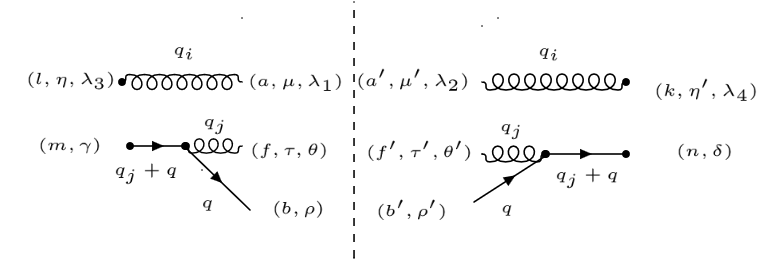
\includegraphics[scale=0.7]{images/GQ/M2Squer.png}
\end{figure}

\begin{equation}
\begin{split}
|M_2|^2=-\frac{{g_s}^2 C_F}{4(k_1 \cdot q_k)(k_1 \cdot q_k)}[(\not{q_k}+\not{k_1}) {\gamma}_{{\tau}^{\prime}}\not{k_1}{\gamma}^{\tau}(\not{q_k}+\not{k_1})][-g^{{\eta}{\eta}^{\prime}}]
\end{split}
\end{equation}

\begin{equation}
\begin{split}
|M_2|^2=(d-2)\frac{{g_s}^2 C_F}{4(k_1 \cdot q_k)}[\not{q_k}][-g^{{\eta}{\eta}^{\prime}}]
\end{split}
\end{equation}

It doesn't contribute to the final result!!

\begin{figure}[ht!]
\centering
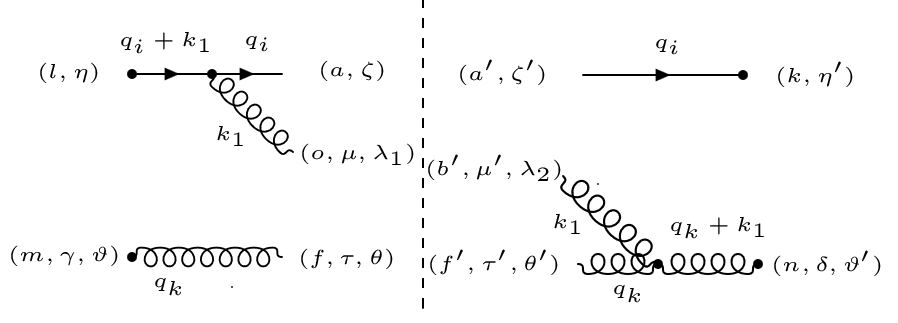
\includegraphics[scale=0.7]{images/GQ/M1M2DaggerGluon.png}
\end{figure}

\begin{equation}
\begin{split}
&M1{M_2}^{\dagger}=\frac{-{g_s}^2 {[T^{o}]_a}^{l} f^{\:f^{\prime}\: b^{\prime}\:n}}{4(k_1 \cdot q_i)(k_1 \cdot q_k)}[\not{q_i}{\gamma}_{\mu}(\not{k_1}+\not{q_i})\:]\\
&[ (g^{{{\gamma}}{{\mu}}}(q_k-k_1)^{\delta}+g^{{{\mu}}{{\delta}}}(2k_1 +q_k)^{{\gamma}}-g^{\delta{{\gamma}}}(2q_k+k_1)^{{\mu}})]\\
\end{split}
\end{equation}

\begin{equation}
\begin{split}
&M1{M_2}^{\dagger}=\frac{-{g_s}^2 {[T^{o}]_a}^{l} f^{\:f^{\prime}\: b^{\prime}\:n}}{4(k_1 \cdot q_i)(k_1 \cdot q_k)}[-\gamma_{\mu}\not{q_i}\not{k_1+2}(\not{k_1}+\not{q_i}){q_i}_{\mu}\:]\\
&[ g^{{{\gamma}}{{\mu}}}(q_k-k_1)^{\delta}+g^{{{\mu}}{{\delta}}}(2k_1+q_k )^{{\gamma}}-g^{\delta{{\gamma}}}(2q_k+k_1)^{{\mu}}]\\
\end{split}
\end{equation}

\begin{equation}
\begin{split}
&M1{M_2}^{\dagger}=\frac{-{g_s}^2 {[T^{o}]_a}^{l} f^{\:f^{\prime}\: b^{\prime}\:n}}{4 y(1-\beta_1) (1-y)\:(p_i \cdot p_k)(p_i \cdot Q)}\\
&[-\gamma_{\mu}((\beta_1 -\alpha_1 y(\frac{Q^2}{2p_i \cdot Q}))\not{p_i} + y\alpha_1\not{Q})((\alpha_1 -y\beta_1(\frac{Q^2}{2p_i \cdot Q})) \not{p_i} + y\beta_1\not{Q})\\
&+(2((\alpha_1 -y\beta_1(\frac{Q^2}{2p_i \cdot Q})) \not{p_i} + 2y\beta_1\not{Q}+2(\beta_1 -\alpha_1 y(\frac{Q^2}{2p_i \cdot Q}))\not{p_i} + 2y\alpha_1\not{Q})(\beta_1{q_i}_{\mu})\:]\\
&[ g^{{{\gamma}}{{\mu}}}(-\alpha_1p_i)^{\delta}+g^{{{\mu}}{{\delta}}}(2\alpha_1p_i )^{{\gamma}}-g^{\delta{{\gamma}}}(\alpha_1p_i+(2-y)Q)^{{\mu}}]\\
\end{split}
\end{equation}

\begin{equation}
\begin{split}
&M1{M_2}^{\dagger}=\frac{-{g_s}^2 C_F}{4 y(1-\beta_1) (1-y)\:(p_i \cdot p_k)(p_i \cdot Q)}\\
&[-\gamma_{\mu}(y\beta_1^2)\not{p_i}\not{Q}+2(\not{p_i}+y\not{Q})(\beta_1{p_i}_{\mu})\:]\\
&[ g^{{{\gamma}}{{\mu}}}(-\alpha_1p_i+\sqrt{1-y} p_k)^{\delta}+g^{{{\mu}}{{\delta}}}(2\alpha_1p_i+ \sqrt{1-y} p_k)^{{\gamma}}-g^{\delta{{\gamma}}}(\alpha_1p_i+2\sqrt{1-y} p_k)^{{\mu}}]\\
\end{split}
\end{equation}

\begin{equation}
\begin{split}
&M1{M_2}^{\dagger}=\frac{-{g_s}^2 C_F}{4 y(1-\beta_1) (1-y)\:(p_i \cdot p_k)(p_i \cdot Q)}\\
&[-\gamma_{\mu}(y\beta_1^2)\not{p_i}\not{Q}][ g^{{{\gamma}}{{\mu}}}(-\alpha_1p_i+\sqrt{1-y} p_k)^{\delta}+g^{{{\mu}}{{\delta}}}(2\alpha_1p_i+ \sqrt{1-y} p_k)^{{\gamma}}-g^{\delta{{\gamma}}}(\alpha_1p_i+2\sqrt{1-y} p_k)^{{\mu}}]\\
&+[2(\not{p_i}+y\not{Q})(\beta_1{p_i}_{\mu})\:][ g^{{{\gamma}}{{\mu}}}(-\alpha_1p_i+\sqrt{1-y} p_k)^{\delta}+g^{{{\mu}}{{\delta}}}(2\alpha_1p_i+ \sqrt{1-y} p_k)^{{\gamma}}-g^{\delta{{\gamma}}}(\alpha_1p_i+2\sqrt{1-y} p_k)^{{\mu}}]\\
\end{split}
\end{equation}

\begin{equation}
\begin{split}
&M1{M_2}^{\dagger}=\frac{-{g_s}^2 C_F}{4 y(1-\beta_1) (1-y)\:(p_i \cdot p_k)(p_i \cdot Q)}\\
&[-\gamma_{\mu}(y\beta_1^2)\not{p_i}\not{Q}][ g^{{{\gamma}}{{\mu}}}(-\alpha_1p_i)^{\delta}+g^{{{\mu}}{{\delta}}}(\alpha_1p_i )^{{\gamma}}-g^{\delta{{\gamma}}}((2-y)Q)^{{\mu}}][{g^{\delta}}_{\gamma}]\\
&+[2\beta_1(\not{p_i}+y\not{Q})\:][{p_i}^{\gamma} (-\alpha_1p_i)^{\delta}+{p_i}^{\delta}(2\alpha_1p_i )^{{\gamma}}-g^{\delta{{\gamma}}}(\alpha_1p_i+(2-y))Q\cdot p_i]\\
\end{split}
\end{equation}

\begin{equation}
\begin{split}
&M1{M_2}^{\dagger}=\frac{-{g_s}^2 C_F}{4 y(1-\beta_1) (1-y)\:(p_i \cdot p_k)(p_i \cdot Q)}\\
&[-\gamma_{\mu}(y\beta_1^2)\not{p_i}\not{Q}][-g^{\delta{{\gamma}}}(\alpha_1p_i+2\sqrt{1-y} p_k)^{{\mu}}]\\
&+[2\beta_1(\not{p_i}+y\not{Q})\:][-g^{\delta{{\gamma}}}(\alpha_1p_i+2\sqrt{1-y})p_i\cdot p_k]\\
\end{split}
\end{equation}

\begin{equation}
\begin{split}
&M1{M_2}^{\dagger}=\frac{-{g_s}^2 C_F}{4 y(1-\beta_1) (1-y)\:(p_i \cdot p_k)(p_i \cdot Q)}\\
&[-2y\beta_1^2\sqrt{1-y} \not{p_k}\not{p_i}\not{Q}+4\sqrt{1-y}\beta_1(\not{p_i}+y\not{Q})p_i\cdot p_k][-g^{\delta{{\gamma}}}]\\
\end{split}
\end{equation}

\begin{equation}
\begin{split}
&M1{M_2}^{\dagger}=\frac{-{g_s}^2 C_F}{y(1-\beta_1) (1-y)\:(p_i \cdot Q)}\sqrt{1-y}\beta_1[\not{p_i}][-g^{\delta{{\gamma}}}]\\
\end{split}
\end{equation}

\subsection{Interpretation of the result}

\begin{equation}
\begin{split}
&|M|^{2}=\frac{-{g_s}^2 C_F}{2y (1-y)\:(p_i \cdot Q)}[\not{p_i}][-g^{\delta{{\gamma}}}]\otimes [2RE(\frac{2\beta_1}{1-\beta_1})+(d-2)(1-\beta_1)]\\
\end{split}
\end{equation}

















